%!Mode:: "TeX:UTF-8"
\documentclass[a4paper,11pt,UTF8]{ctexart}

\usepackage{indentfirst} %缩进
\usepackage{xeCJK}    %使用系统字体
\usepackage{fancyhdr} %自定义页眉页脚
\pagestyle{empty}                   %不设置页眉页脚
\usepackage{amsmath, amsthm, amssymb, amsfonts} %数学公式
\usepackage[a4paper,left=3cm,right=3cm,top=3cm,bottom=3cm]{geometry}
%\usepackage[tmargin=1in,bmargin=1in,lmargin=1.25in,rmargin=1.25in]{geometry}.
\usepackage{booktabs} %插入表格
\usepackage[section]{placeins} %避免浮动
\usepackage{listings} %插入代码
\usepackage{ctex}     %中文宏包
\usepackage[svgnames, table]{xcolor} %彩色表格
\usepackage{algorithm}          %伪代码
\usepackage{algorithmicx}
\usepackage{algpseudocode}
\usepackage{algorithm,algpseudocode,float}
\usepackage{lipsum}
\usepackage{enumitem}           %调整列举环境
\usepackage{url}
\usepackage{fontspec,xunicode}
\usepackage{upgreek}
\defaultfontfeatures{Mapping=tex-text} %如果没有它,会有一些 tex 特殊字符无法正常使用,比如连字符。

\usepackage{graphicx}
\graphicspath{{imgs/}}

%%%%%%%%%%%%%%%%%%%%%%%%%%%%%%%%%%%%%%%%%%%%%%%%%%%%%%%%%%%%%%%%
% 缩进及行间距
%%%%%%%%%%%%%%%%%%%%%%%%%%%%%%%%%%%%%%%%%%%%%%%%%%%%%%%%%%%%%%%%
\setlength{\parindent}{22pt} %重新定义缩进长度
\setlength{\baselineskip}{20pt}  %定义行间距
%\renewcommand{\baselinestretch}{1.1} %定义行间距

%%%%%%%%%%%%%%%%%%%%%%%%%%%%%%%%%%%%%%%%%%%%%%%%%%%%%%%%%%%%%%%%
% 列表设置
%%%%%%%%%%%%%%%%%%%%%%%%%%%%%%%%%%%%%%%%%%%%%%%%%%%%%%%%%%%%%%%%
\setenumerate{fullwidth,itemindent=\parindent,listparindent=\parindent,itemsep=0ex,partopsep=0pt,parsep=0ex}
\setenumerate[2]{label=\alph*),leftmargin=1.5em}  %二级item设置
\setitemize{itemindent=38pt,leftmargin=0pt,itemsep=-0.4ex,listparindent=26pt,partopsep=0pt,parsep=0.5ex,topsep=-0.25ex}
\setdescription{itemindent=38pt,leftmargin=0pt,itemsep=-0.4ex,listparindent=26pt,partopsep=0pt,parsep=0.5ex,topsep=-0.25ex}

%%%%%%%%%%%%%%%%%%%%%%%%%%%%%%%%%%%%%%%%%%%%%%%%%%%%%%%%%%%%%%%%
% 图的标题行间距设置
%%%%%%%%%%%%%%%%%%%%%%%%%%%%%%%%%%%%%%%%%%%%%%%%%%%%%%%%%%%%%%%%
\newcommand{\bottomcaption}{%
\setlength{\abovecaptionskip}{6pt}%
\setlength{\belowcaptionskip}{6pt}%
\caption}


%%%%%%%%%%%%%%%%%%%%%%%%%%%%%%%%%%%%%%%%%%%%%%%%%%%%%%%%%%%%%%%%
% 字体定义
%%%%%%%%%%%%%%%%%%%%%%%%%%%%%%%%%%%%%%%%%%%%%%%%%%%%%%%%%%%%%%%%
\setmainfont{Times New Roman}  %默认英文字体.serif是有衬线字体sans serif无衬线字体
\setmonofont{Consolas}
\setCJKmainfont[ItalicFont={楷体}, BoldFont={黑体}]{宋体}%衬线字体 缺省中文字体为
\setCJKsansfont{黑体}
\punctstyle{hangmobanjiao}
%-----------------------xeCJK下设置中文字体------------------------------%
\setCJKfamilyfont{song}{SimSun}                             %宋体 song
\newcommand{\song}{\CJKfamily{song}}
\setCJKfamilyfont{fs}{FangSong}                      %仿宋  fs
\newcommand{\fs}{\CJKfamily{fs}}
\setCJKfamilyfont{ktgb}{KaiTi}                      %楷体2312 ktgb
\newcommand{\ktgb}{\CJKfamily{ktgb}}
\setCJKfamilyfont{yh}{Microsoft YaHei}                    %微软雅黑 yh
\newcommand{\yh}{\CJKfamily{yh}}
\setCJKfamilyfont{hei}{SimHei}                              %黑体  hei
\newcommand{\hei}{\CJKfamily{hei}}
\setCJKfamilyfont{hwxk}{STXingkai}                                %华文行楷  hwxk
\newcommand{\hwxk}{\CJKfamily{hwxk}}
%------------------------------设置字体大小------------------------%
\newcommand{\shiyanbaogao}{\fontsize{36pt}{\baselineskip}\selectfont}
\newcommand{\chuhao}{\fontsize{42pt}{\baselineskip}\selectfont}     %初号
\newcommand{\xiaochuhao}{\fontsize{36pt}{\baselineskip}\selectfont} %小初号
\newcommand{\yihao}{\fontsize{28pt}{\baselineskip}\selectfont}      %一号
\newcommand{\erhao}{\fontsize{21pt}{\baselineskip}\selectfont}      %二号
\newcommand{\xiaoerhao}{\fontsize{18pt}{\baselineskip}\selectfont}  %小二号
\newcommand{\sanhao}{\fontsize{15.75pt}{\baselineskip}\selectfont}  %三号
\newcommand{\sihao}{\fontsize{14pt}{\baselineskip}\selectfont}       %四号
\newcommand{\xiaosihao}{\fontsize{12pt}{\baselineskip}\selectfont}  %小四号
\newcommand{\wuhao}{\fontsize{10.5pt}{\baselineskip}\selectfont}    %五号
\newcommand{\xiaowuhao}{\fontsize{9pt}{\baselineskip}\selectfont}   %小五号
\newcommand{\liuhao}{\fontsize{7.875pt}{\baselineskip}\selectfont}  %六号
\newcommand{\qihao}{\fontsize{5.25pt}{\baselineskip}\selectfont}    %七号

%%%%%%%%%%%%%%%%%%%%%%%%%%%%%%%%%%%%%%%%%%%%%%%%%%%%%%%%%%%%%%%%
% 图题字体大小相同
%%%%%%%%%%%%%%%%%%%%%%%%%%%%%%%%%%%%%%%%%%%%%%%%%%%%%%%%%%%%%%%%
\usepackage{caption}
\captionsetup{font={footnotesize}}   % footnotesize = 9pt
\captionsetup[lstlisting]{font={footnotesize}}

%%%%%%%%%%%%%%%%%%%%%%%%%%%%%%%%%%%%%%%%%%%%%%%%%%%%%%%%%%%%%%%%
% 重定义枚举编号为 1),2)...
%%%%%%%%%%%%%%%%%%%%%%%%%%%%%%%%%%%%%%%%%%%%%%%%%%%%%%%%%%%%%%%%
\renewcommand{\labelenumi}{\theenumi)}

%%%%%%%%%%%%%%%%%%%%%%%%%%%%%%%%%%%%%%%%%%%%%%%%%%%%%%%%%%%%%%%%
% 标题名称中文化
%%%%%%%%%%%%%%%%%%%%%%%%%%%%%%%%%%%%%%%%%%%%%%%%%%%%%%%%%%%%%%%%
\renewcommand\figurename{\hei 图}
\renewcommand\tablename{\hei 表}
\renewcommand\lstlistingname{\hei 代码}
\renewcommand{\algorithmicrequire}{\textbf{输入:}}
\renewcommand{\algorithmicensure}{\textbf{输出:}}
\newtheorem{define}{定义}

%%%%%%%%%%%%%%%%%%%%%%%%%%%%%%%%%%%%%%%%%%%%%%%%%%%%%%%%%%%%%%%%
% 代码设置
%%%%%%%%%%%%%%%%%%%%%%%%%%%%%%%%%%%%%%%%%%%%%%%%%%%%%%%%%%%%%%%%
\lstset{
 columns=fixed,
 numbers=left,                                        % 在左侧显示行号
 numberstyle=\tiny\color{gray},                       % 设定行号格式
 frame=single,                                        % 单线背景边框
 breaklines=true,                                     % 设定LaTeX对过长的代码行进行自动换行
 keywordstyle=\color[RGB]{40,40,255},                 % 设定关键字颜色
 numberstyle=\footnotesize\color{darkgray},
 commentstyle=\it\color[RGB]{0,96,96},                % 设置代码注释的格式
 stringstyle=\rmfamily\slshape\color[RGB]{128,0,0},   % 设置字符串格式
 showstringspaces=false,                              % 不显示字符串中的空格
 language=java,                                        % 设置语言
 basicstyle=\linespread{1.0}\xiaowuhao\ttfamily,                      % 字体字号
 %lineskip=10pt,
 %baselinestretch=1,
}

%%%%%%%%%%%%%%%%%%%%%%%%%%%%%%%%%%%%%%%%%%%%%%%%%%%%%%%%%%%%%%%%
% 伪代码分页
%%%%%%%%%%%%%%%%%%%%%%%%%%%%%%%%%%%%%%%%%%%%%%%%%%%%%%%%%%%%%%%%
\makeatletter
\renewcommand{\ALG@name}{算法}
\newenvironment{breakablealgorithm}
  {% \begin{breakablealgorithm}
   \begin{center}
     \refstepcounter{algorithm}% New algorithm
     \hrule height.8pt depth0pt \kern2pt% \@fs@pre for \@fs@ruled
     \renewcommand{\caption}[2][\relax]{% Make a new \caption
       {\raggedright\textbf{\ALG@name~\thealgorithm} ##2\par}%
       \ifx\relax##1\relax % #1 is \relax
         \addcontentsline{loa}{algorithm}{\protect\numberline{\thealgorithm}##2}%
       \else % #1 is not \relax
         \addcontentsline{loa}{algorithm}{\protect\numberline{\thealgorithm}##1}%
       \fi
       \kern2pt\hrule\kern2pt
     }
  }{% \end{breakablealgorithm}
     \kern2pt\hrule\relax% \@fs@post for \@fs@ruled
   \end{center}
  }
\makeatother

% =============================================
% Part 1 Edit the info
% =============================================

\newcommand{\major}{物理学院}
\newcommand{\name}{黄阅迅,李秋阳}
\newcommand{\stuid}{PB18020631,PB18020567}
\newcommand{\group}{20}
\newcommand{\newdate}{\today}


\newcommand{\course}{电子线路实验(1)}
\newcommand{\newtitle}{二极管的基本应用}

% =============================================
% Part 1 Main document
% =============================================
\begin{document}
\thispagestyle{empty}
\begin{figure}[h]
  \begin{minipage}{0.6\linewidth}
    \centerline{
\includegraphics[width=\linewidth]{logo.png}}
  \end{minipage}
  \hfill
  \begin{minipage}{.4\linewidth}
    \raggedleft
    \begin{tabular*}{.8\linewidth}{ll}
      学院: & \underline\major   \\
      姓名: & \underline\name    \\
      学号: & \underline\stuid   \\
      组号:  & \underline\group   \\
      日期: & \underline\newdate \\
    \end{tabular*}
  \end{minipage}
\end{figure}

\begin{table}[!htbp]
  \centering
  \begin{tabular*}{\linewidth}{llllll}
    课程名称:  \underline\course   \qquad\qquad 实验题目:  \underline\newtitle  
  \end{tabular*}
\end{table}

%
\newcommand\mr[1]{\mathrm{#1}}
\newcommand\dd{\mathrm{d\,}}
% =============================================
% Part 2 Main document
% =============================================

\section{实验目的}

参看预习报告。

\section{实验原理}

部分内容参看预习报告。以下为补充内容。

\subsection{整流滤波电路}
如图 \ref{fig:SVCsim}为最简单的整流电路,其中包含一个二极管与负载电阻$R_L$,当正板周期时,二极管导通,负半周时,二极管截止。
由此达到整流目的,其输出波形如图右侧所示。
\begin{figure}[htbp]
  \centering
  \fbox{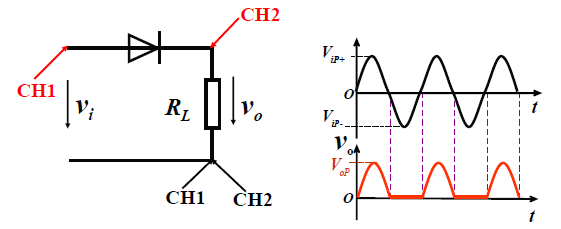
\includegraphics[width=0.5\linewidth]{SVCsim}}
  \caption{整流电路电路与波形示意图}
  \label{fig:SVCsim}
  \end{figure}
则理论上可以计算出输出电压的平均值为
\begin{equation}
  \bar{V}_0=\frac{1}{T}\int_0^Tv_0(t)dt=\frac{V_p}{\pi}\approx0.318V_p
\label{eqa:avgV_SVC}
\end{equation}
当并联电容时,电容的阻抗随频率增大而减小,因此可以起到一定的滤高频波的作用,其电路图及波形如图 \ref{fig:SVCcom}所示。
\begin{figure}[htbp]
  \centering
  \fbox{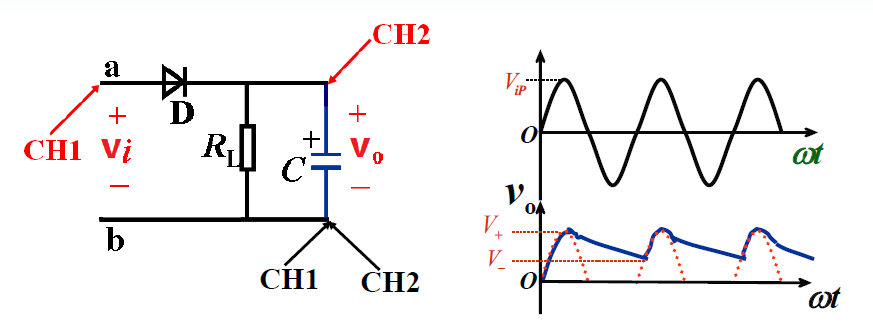
\includegraphics[width=0.5\linewidth]{SVCcom}}
  \caption{整流滤波电路电路与波形示意图}
  \label{fig:SVCcom}
  \end{figure}

\subsection{钳位电路}
其电路与波形如图 \ref{fig:clamper}所示。二极管作理想处理,当输入正弦波时,当$V_i$上升到$E$时,二极管D导通,$V_o$就不可能再上升,被钳位
在这一电平上。$V_i$继续上升,多余的电压被充到电容C上,由于二极管正向导通电阻很小,充电很快,电容电压可充到$V_p-E$。
当$V_i$电压从峰值下降时,二极管截止,输出电压$V_o$为电容上电压和$V_i$的代数和。整个波形被压下$V_p-E$伏,顶端被钳制在E上。
但实际上二极管有压降,实际分析时需要考虑二极管压降。
\begin{figure}[htbp]
  \centering
  \fbox{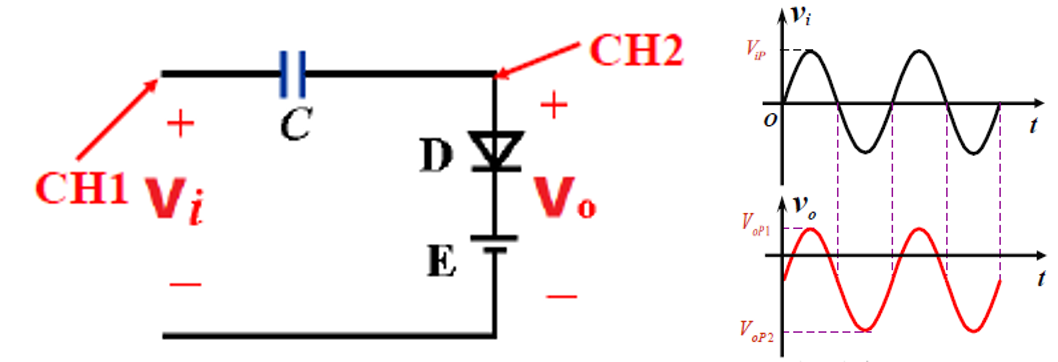
\includegraphics[width=0.5\linewidth]{clamper}}
  \caption{钳位电路电路电路与波形示意图}
  \label{fig:clamper}
  \end{figure}

\subsection{限幅电路}
限幅电路,又称削波电路,是用来限制输出信号电压范围的电路,仅有上门限的称为上限幅
电路,仅有下门限的称为下限幅电路,具有上下门限的限幅电路,称为双向限幅电路。其工作原理与整流电路相近,由于恒压源的存在,使得当输入电压加上恒压源一旦超出了二
极管的导通范围,就会截止,因此具有限制幅度的功能。其电路与输出波形如图 \ref{fig:limiter}所示。二极管作理想处理,当输入正弦波时,输出波形最大值受到限制,相当于顶端被“削平”。
\begin{figure}[htbp]
  \centering
  \fbox{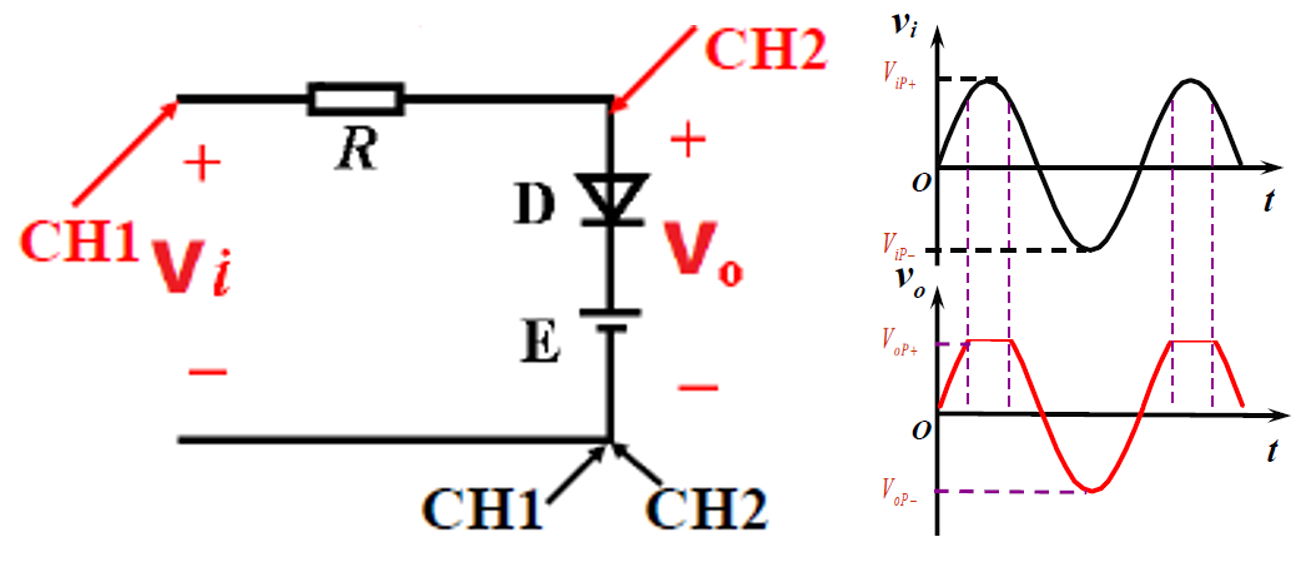
\includegraphics[width=0.5\linewidth]{limiter}}
  \caption{限幅电路电路与波形示意图}
  \label{fig:limiter}
  \end{figure}

\subsection{稳压电路}
其电路图如图 \ref{fig:stabler}所示。当负载$R_L$一定时,如果$V_i$增大,则$V_z$增大,由于稳压二极管动态电阻很小,干路的电流基本上被其捕获,因此$R_1$上的压降增大,最终$V_o$几乎不变。
当$R_L$减小时,则其干路路电流增大,因此干路压降增大,则$V_z$分压减小,最终$V_o$基本不变。
\begin{figure}[htbp]
  \centering
  \fbox{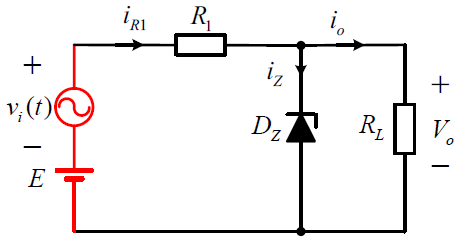
\includegraphics[width=0.5\linewidth]{stabler}}
  \caption{限幅电路电路与波形示意图}
  \label{fig:stabler}
  \end{figure}


\section{实验内容与步骤}
\subsection{实验一:整流滤波电路}
\begin{figure}[H]
 \centering
 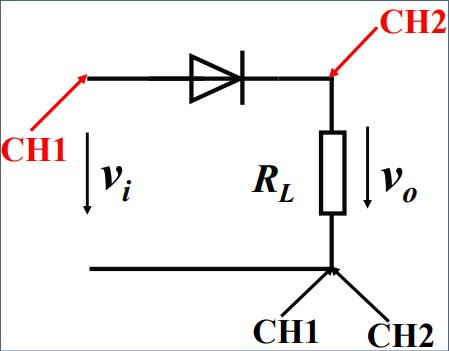
\includegraphics[width=5cm]{Exp1}
 \caption{实验一电路图}
 \label{fig:Exp1}
\end{figure}
如图\ref{fig:Exp1}所示为整流电路。用万用表的两个CH测量其输入和输出电压,再用万用表手动1V DCV档测量其平均值。
\begin{figure}[H]
 \centering
 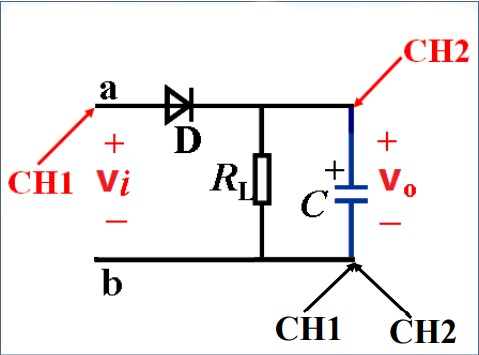
\includegraphics[width=5cm]{Exp1Con}
 \caption{实验一(续)电路图}
 \label{fig:Exp1Con}
\end{figure}
如图\ref{fig:Exp1Con}所示,在图\ref{fig:Exp1}基础上再并联一个电容$C=10\mathrm{\upmu F}$。用示波器测出其输入、输出电压,再用万用表ACV档测量其纹波电压。然后将电容值改为$C=100\mathrm{\upmu F}$,重复实验。
\subsection{实验二:钳位电路}
\begin{figure}[H]
 \centering
 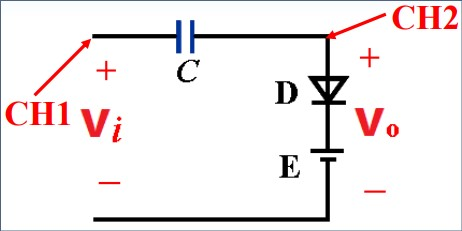
\includegraphics[width=5cm]{Exp2}
 \caption{实验二电路图}
 \label{fig:Exp2}
\end{figure}
如图\ref{fig:Exp2}所示为钳位电路。用示波器测量其输入与输出电压。
\subsection{实验三:限幅电路}
\begin{figure}[H]
 \centering
 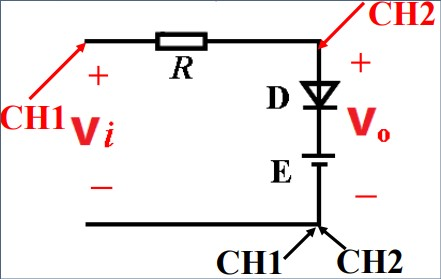
\includegraphics[width=5cm]{Exp3}
 \caption{实验三电路图}
 \label{fig:Exp3}
\end{figure}
如图\ref{fig:Exp3}所示为限幅电路。用示波器测量其输入与输出电压。再用示波器的$X - Y$模式测量其$v_i - v_o$曲线。
\subsection{实验四:稳压电路}
\begin{figure}[H]
 \centering
 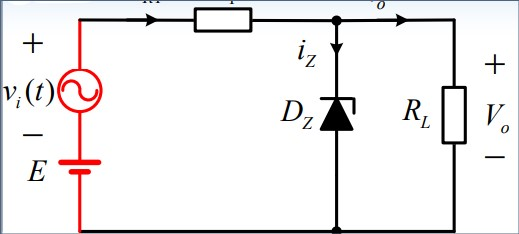
\includegraphics[width=5cm]{Exp4}
 \caption{实验四电路图}
 \label{fig:Exp4}
\end{figure}
如图\ref{fig:Exp4}所示为稳压电路。用示波器测量其输入与输出电压。稳压管等效的交流小信号模型为一个小电阻,用万用表间接测量其等效电路电阻,同时稳压管在静态工作点有一电压降,因此可认为是一反向直流电压源。因此稳压管的等效电路模型是一个小电阻与一个反向直流电源串联。

\section{实验数据处理与分析}
实验所用的普通二极管导通压降为$V_D=0.5823\mr{V}$,稳压二极管的正向导通电压为$V_{DS}=0.7354\mr{V}$。
\subsection{实验一:整流滤波电路}
\begin{figure}[H]
 \centering
 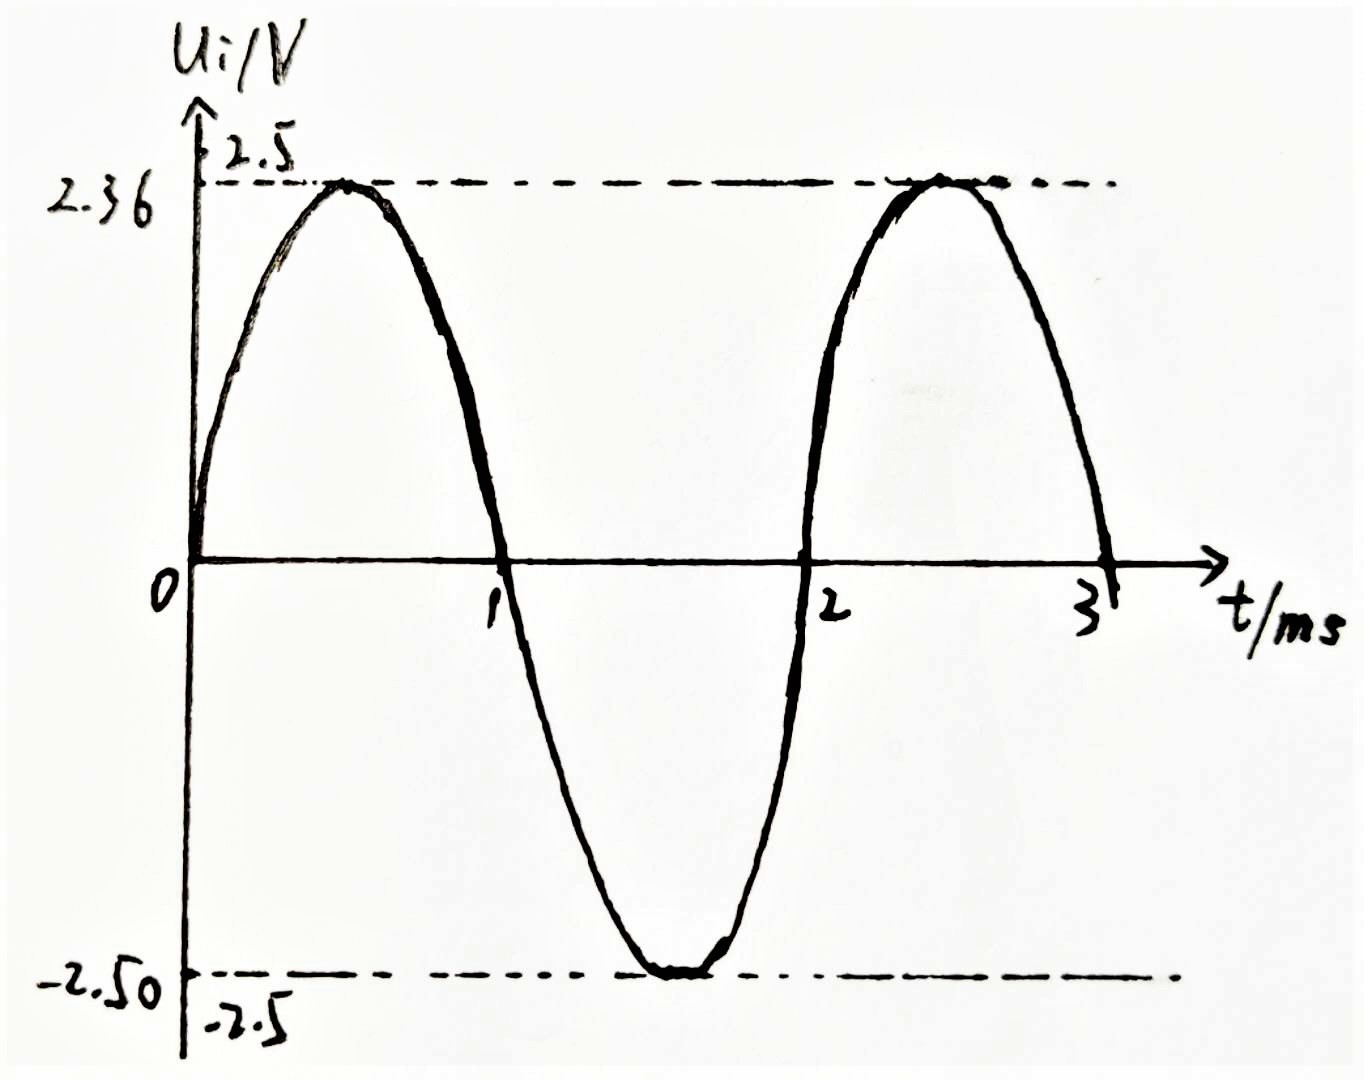
\includegraphics[width=7cm]{Exp1i}
 \caption{实验一输入波形}
 \label{fig:Exp1i}
\end{figure}
在未接电容时,输入波形的高峰值为$V_H=2.36\mr{V}$,低峰值为$V_L=-2.50\mr{V}$,如图\ref{fig:Exp1i}所示。
\begin{figure}[H]
 \centering
 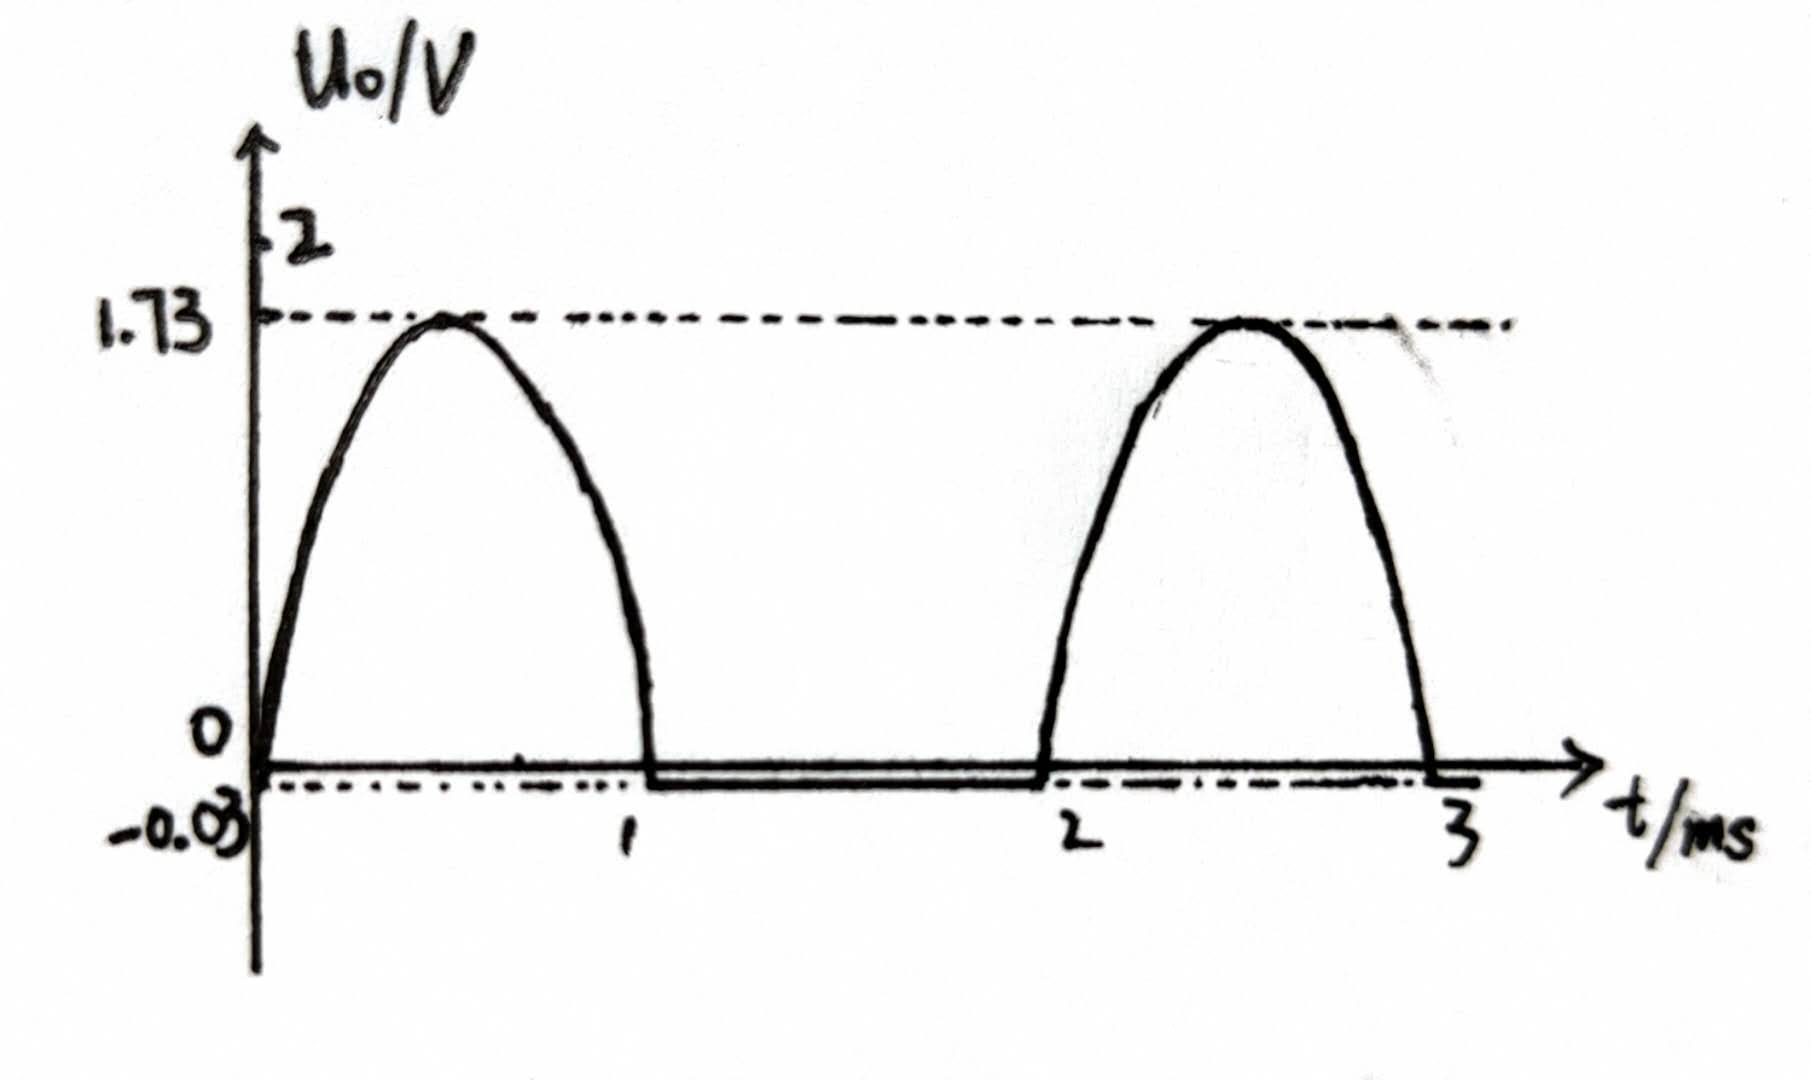
\includegraphics[width=7cm]{Exp1o}
 \caption{实验一输出波形}
 \label{fig:Exp1o}
\end{figure}
在未接电容时,输出波形的高峰值为$V_H=1.73\mr{V}$,低值被削平,为$V_L=-0.03\mr{V}$,如图\ref{fig:Exp1o}。
\par 理论上,峰值电压应为$V_{iH}-V_D=2.36-0.5823=1.778\mr{V}$,与实验值接近,比实验值略大。这可能是由于二极管存在电阻,所以存在分压作用分压作用,电阻实际分到的电压比输入电压略小一些。
\par 万用表测得的平均值为$0.4328\mr{V}$。
而理论给出的平均值为:
\[ \bar{V_o}=\frac{1}{T}\int_0^TV_o(t)\dd{t}\approx0.318V_P=0.318\times1.73=0.55014\mr{V} \]
\par 这个值比实验值大。分析其原因:万用表可能是测量若干个断点的值,并对对应时间内的电压作近似积分。而万用表的采样频率可能没有快到可以精确测量电压平均值,所以在用矩形分割法进行近似积分时有误差。
\begin{figure}[H]
 \centering
 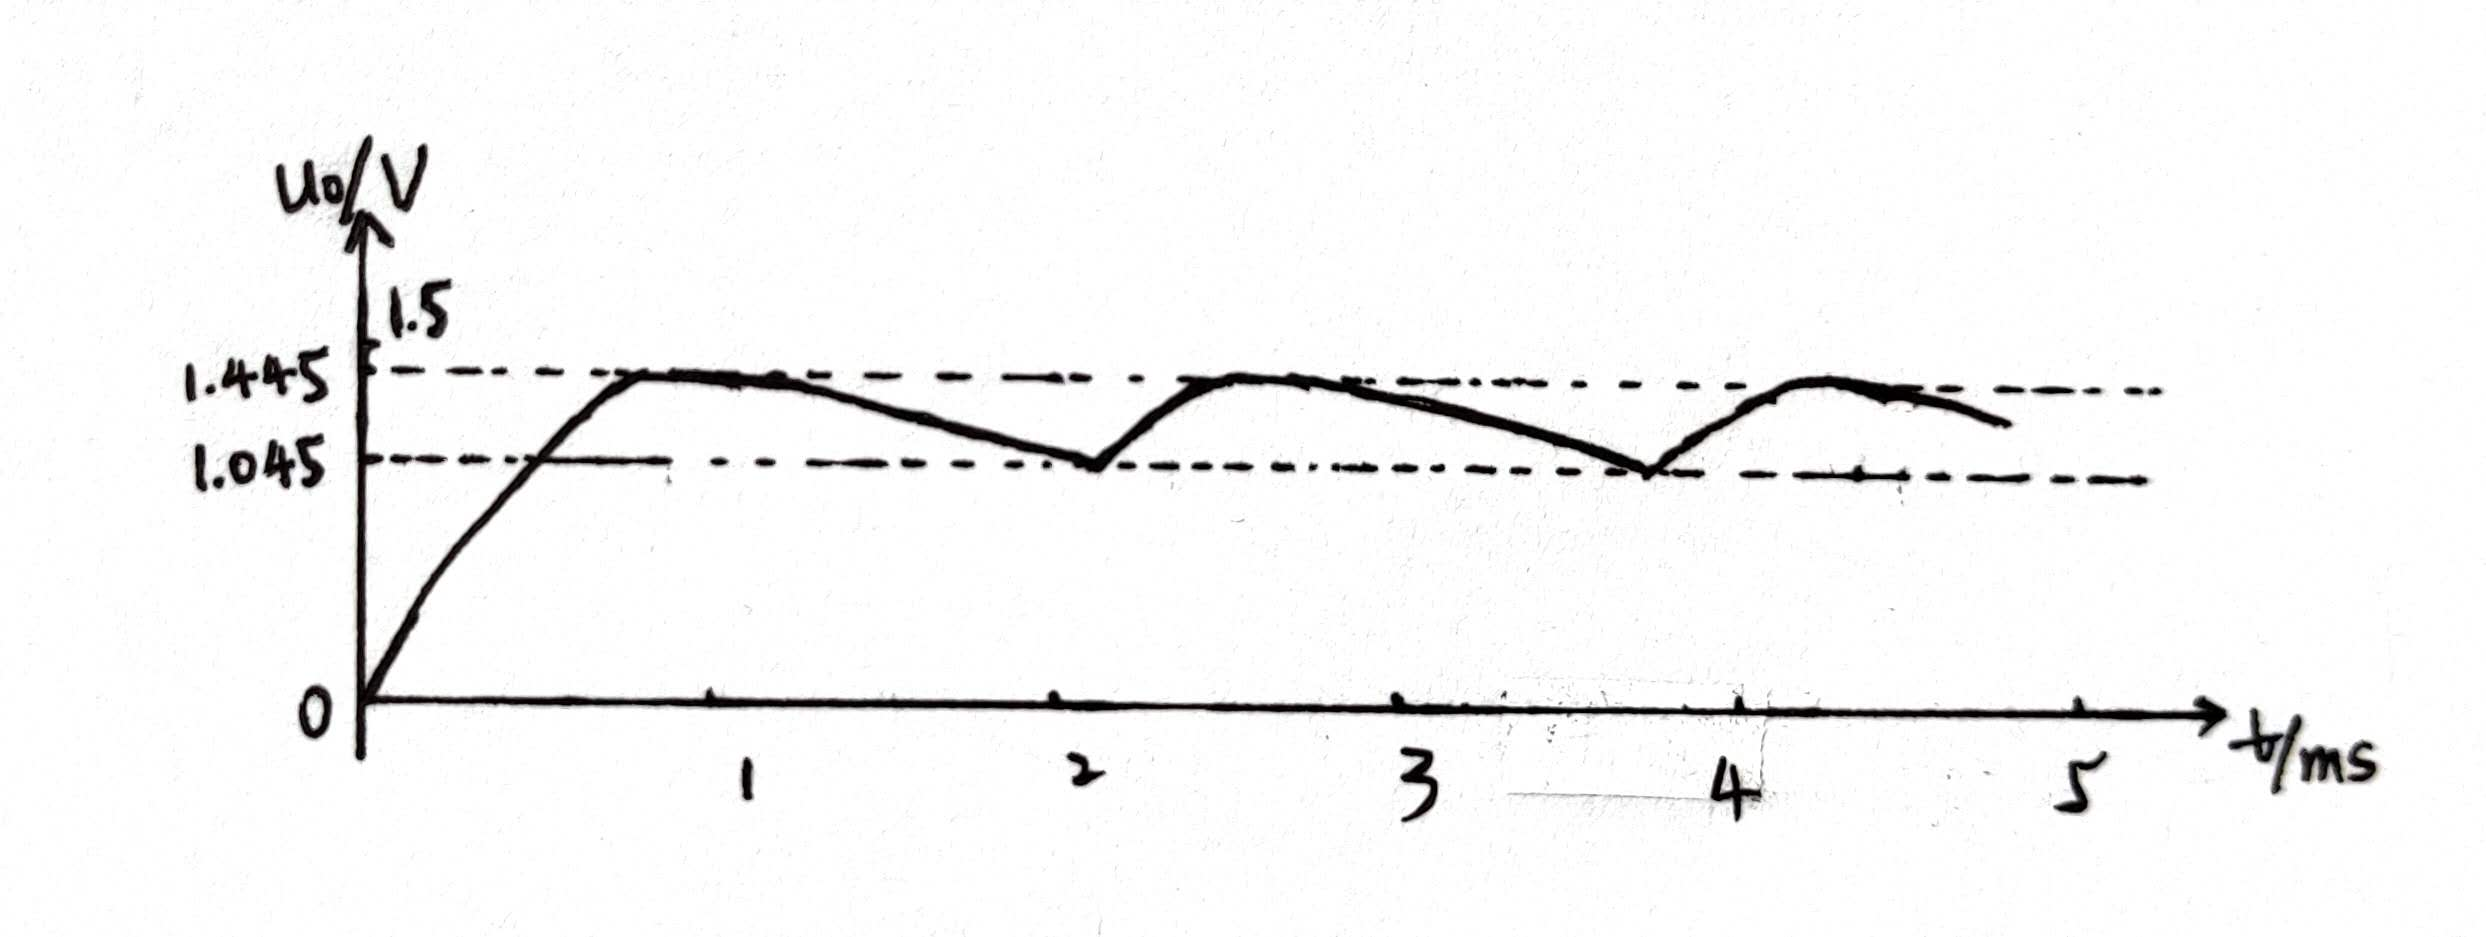
\includegraphics[width=10cm]{Exp1Cono1}
 \caption{实验一(续)输出波形,$C=10\mr{\upmu F}$}
 \label{fig:Exp1Cono1}
\end{figure}
在电容为$10\mr{\mu F}$时,输出波形如图\ref{fig:Exp1Cono1}所示。其中波纹高值为$V_H=1.445\mr{V}$,波纹低值为$V_L=1.043\mr{V}$。
\par 万用表测量的平均值为$\widetilde{V_o}=0.1089\mr{V}$。
\begin{figure}[H]
 \centering
 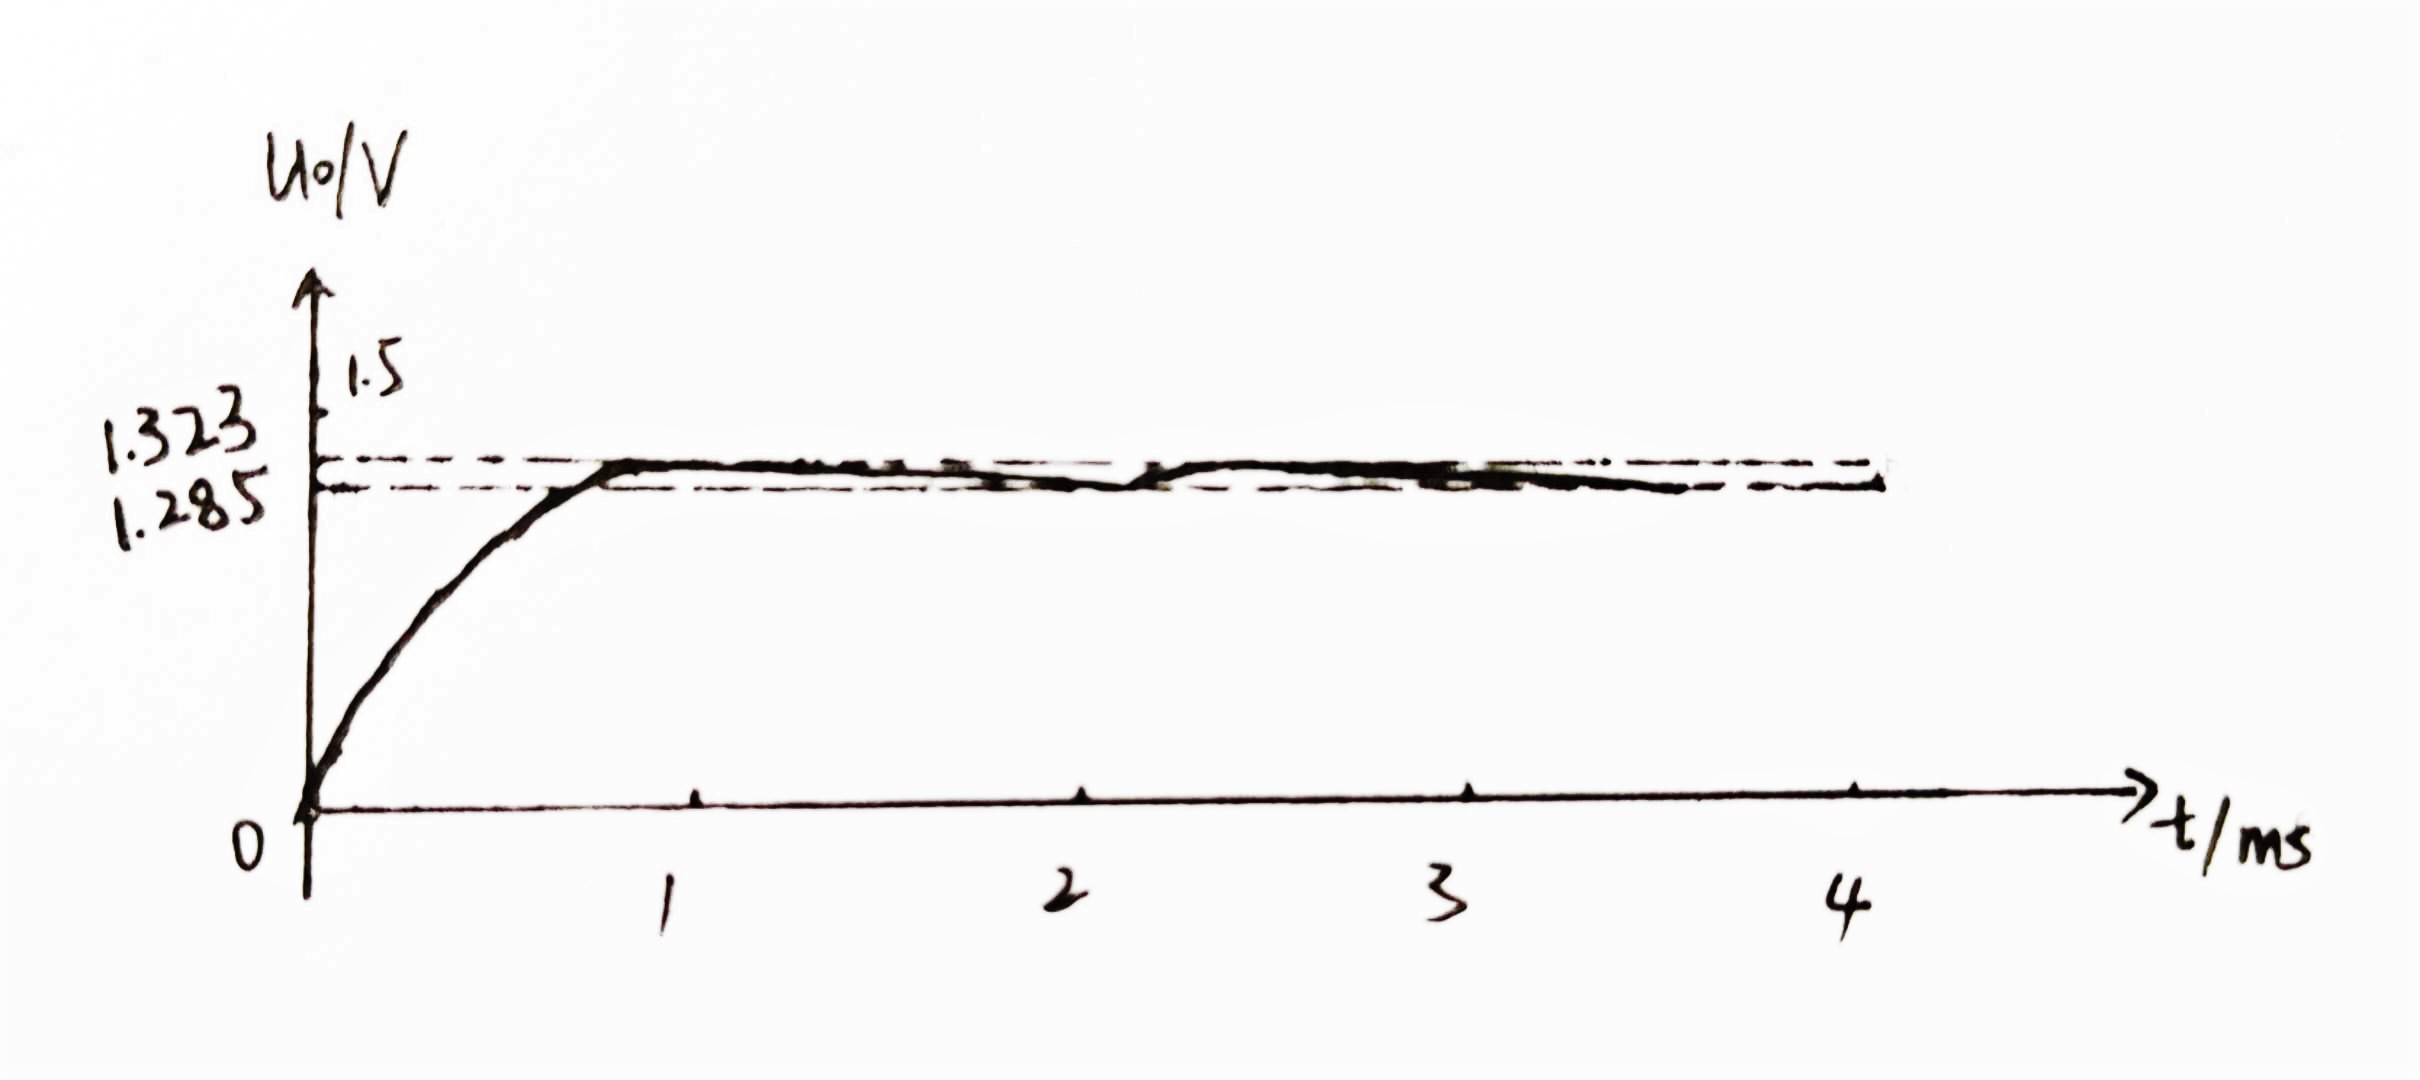
\includegraphics[width=10cm]{Exp1Cono2}
 \caption{实验一(续)输出波形,$C=100\mr{\upmu F}$}
 \label{fig:Exp1Cono2}
\end{figure}
在电容为$100\mr{\mu F}$时,输出波形如图\ref{fig:Exp1Cono2}所示。其中波纹高值为$V_H=1.323\mr{V}$,波纹低值为$V_L=1.285\mr{V}$。
\par 万用表测量的平均值为$\widetilde{V_o}=7.158\mr{mV}$。
\par 比较不同电容值下的结果,我们发现:如果提高电容,那么波纹高值会下降,波纹低值会上升,二者之间差距缩小,所以交流波纹电压减小。
\par 分析其原因:若电容$C=100\mr{\upmu F}$,那么相较于$C=10\mr{\upmu F}$时,电容的阻抗更小了,与负载电阻的并联阻抗也变小了,分压能力减弱,所以波纹高值减小了;而此时电路的时间常数$\tau=RC$更大了,电路中电压的变化更为缓慢,于是第二次实验的波纹更小,因此波纹低值也更高,交流波纹电压更小。
\subsection{实验二:钳位电路}
\begin{figure}[H]
 \centering
 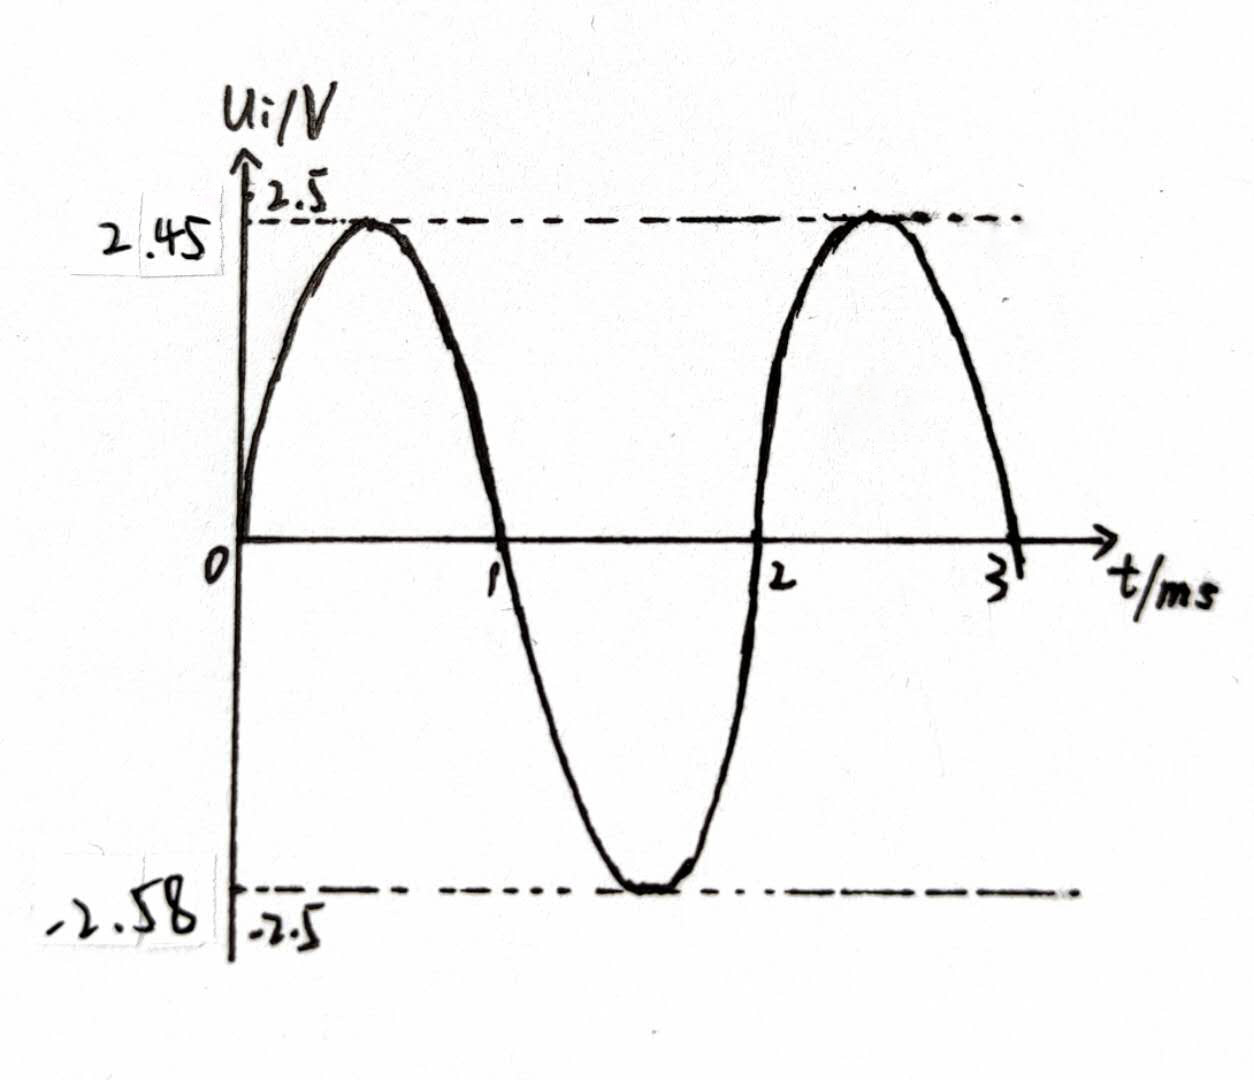
\includegraphics[width=7cm]{Exp2i}
 \caption{实验二输入波形}
 \label{fig:Exp2i}
\end{figure}
实验输入波形如图\ref{fig:Exp2i}所示。高峰值为$V_H=2.45\mr{V}$,低峰值为$V_L=-2.58\mr{V}$。
\begin{figure}[H]
 \centering
 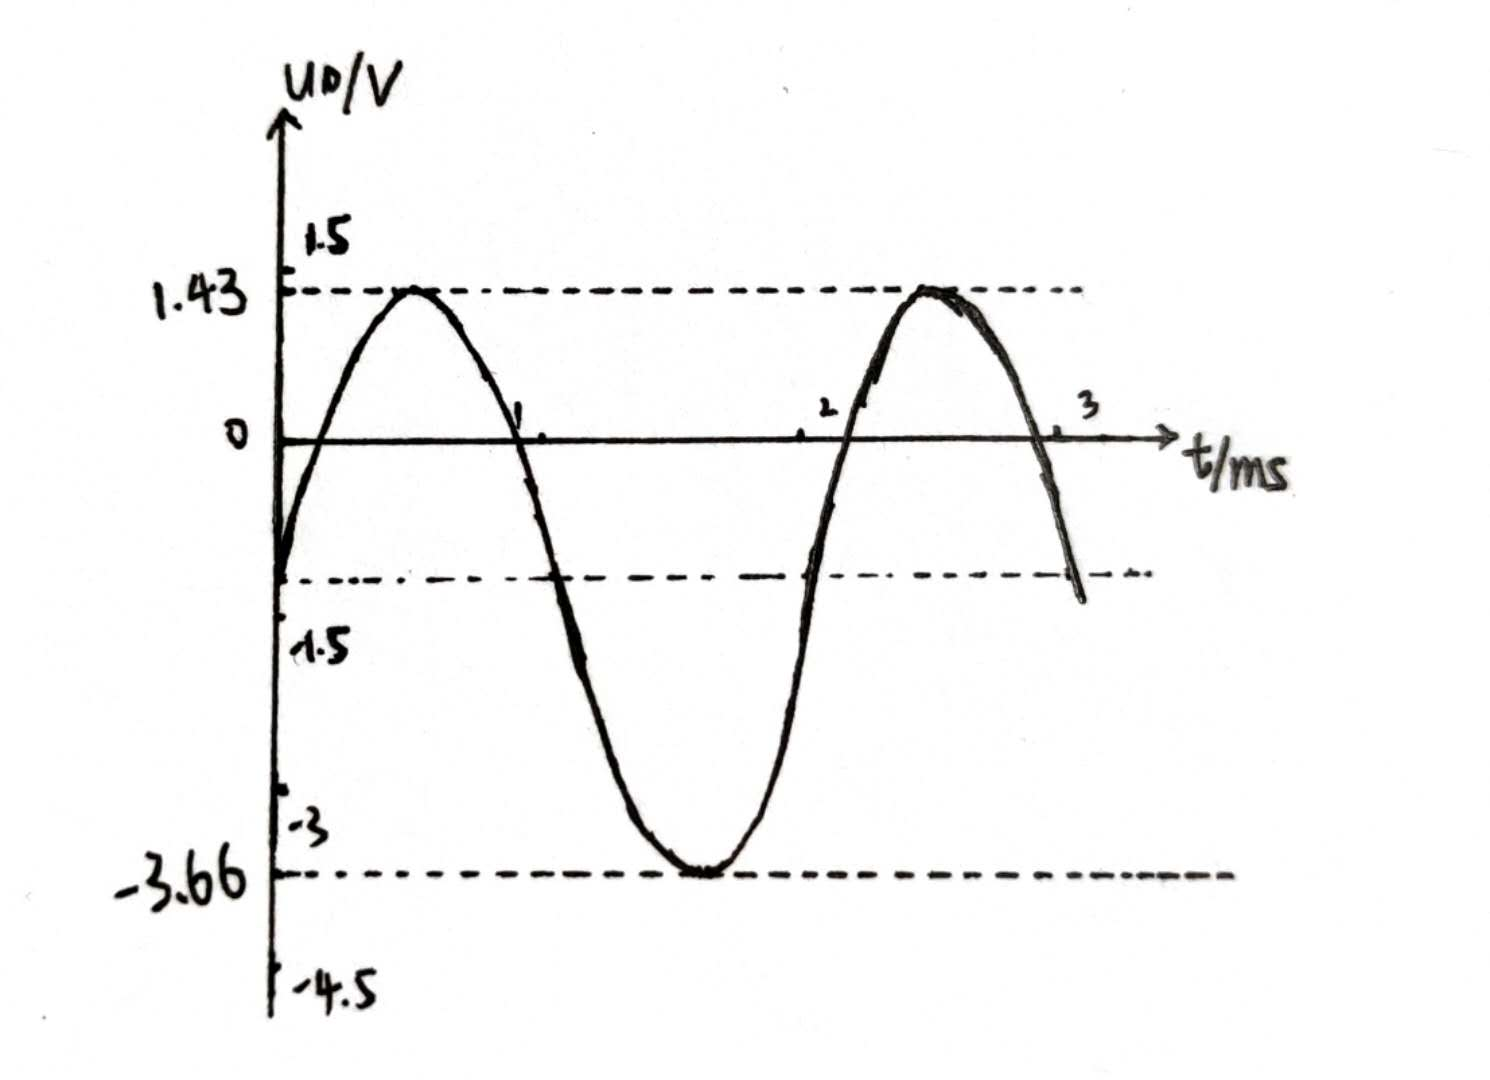
\includegraphics[width=7cm]{Exp2o}
 \caption{实验二输出波形}
 \label{fig:Exp2o}
\end{figure}
实验输出波形如图\ref{fig:Exp2o}所示。高峰值为$V_H=1.43\mr{V}$,低峰值为$V_L=-3.66\mr{V}$。
\par 理论上,输出波形相对于输入波形向下平移了$E=1\mr{V}$,实际上波形的高峰和低峰分别向下平移了$2.45-1.43=1.02\mr{V}$和$-2.58-(-3.66)=1.08\mr{V}$,和理论值符合得比较好。
\subsection{实验三:限幅电路}
\begin{figure}[H]
 \centering
 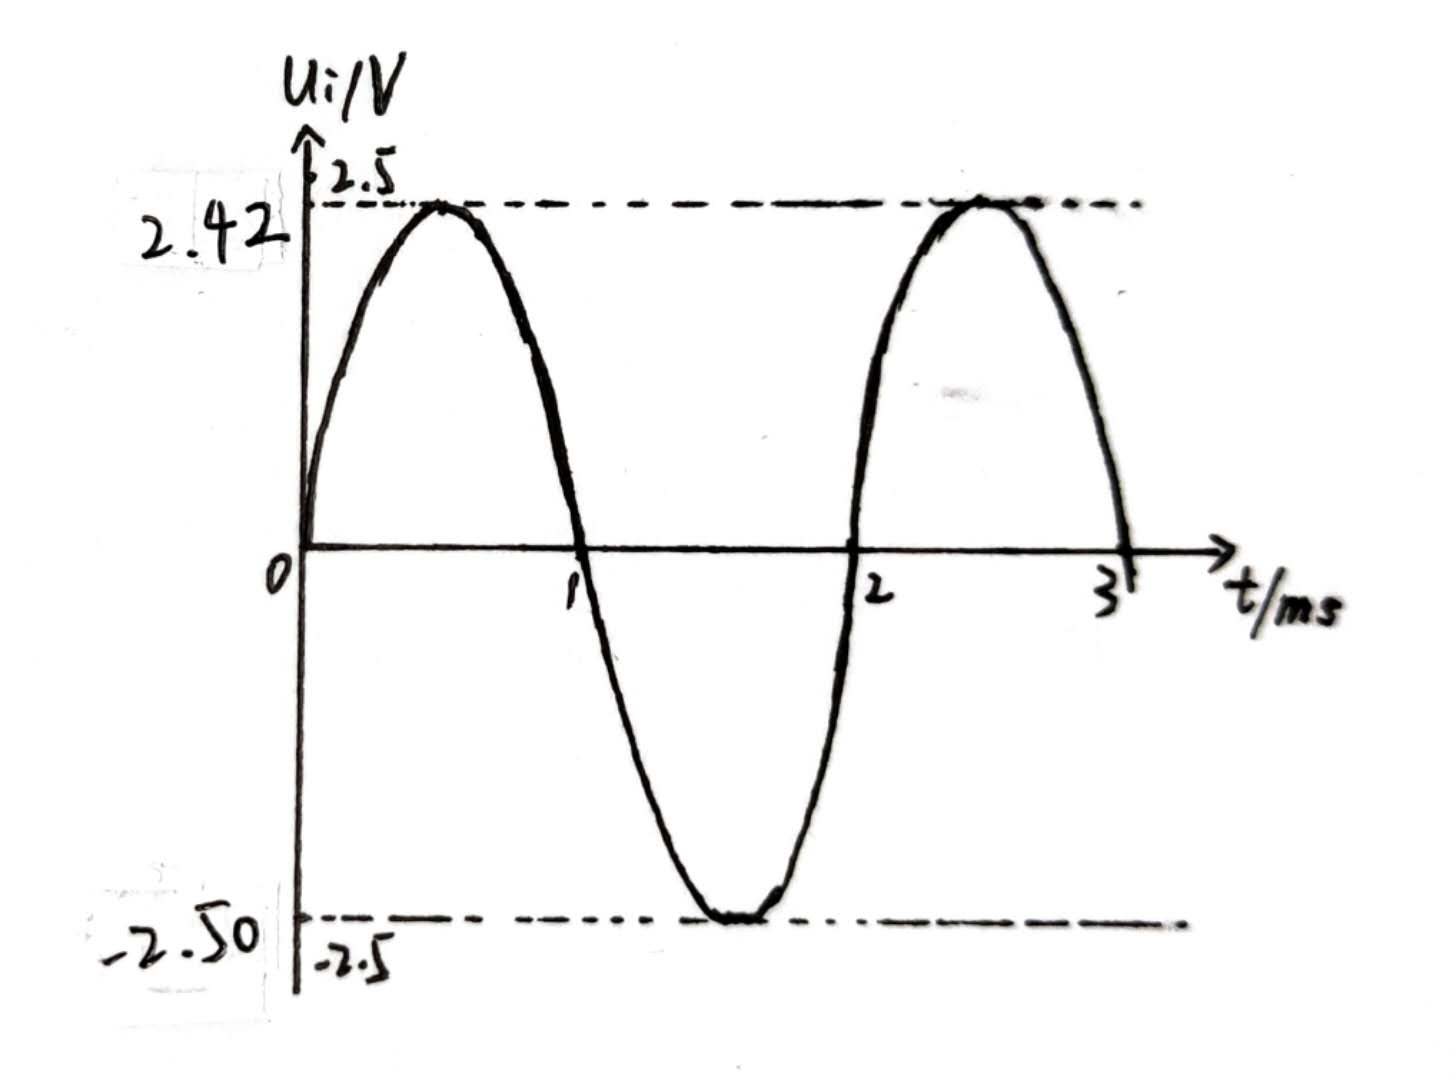
\includegraphics[width=7cm]{Exp3i}
 \caption{实验三输入波形}
 \label{fig:Exp3i}
\end{figure}
实验输入波形如图\ref{fig:Exp3i}所示。高峰值为$V_H=2.42\mr{V}$,低峰值为$V_L=-2.50\mr{V}$。
\begin{figure}[H]
 \centering
 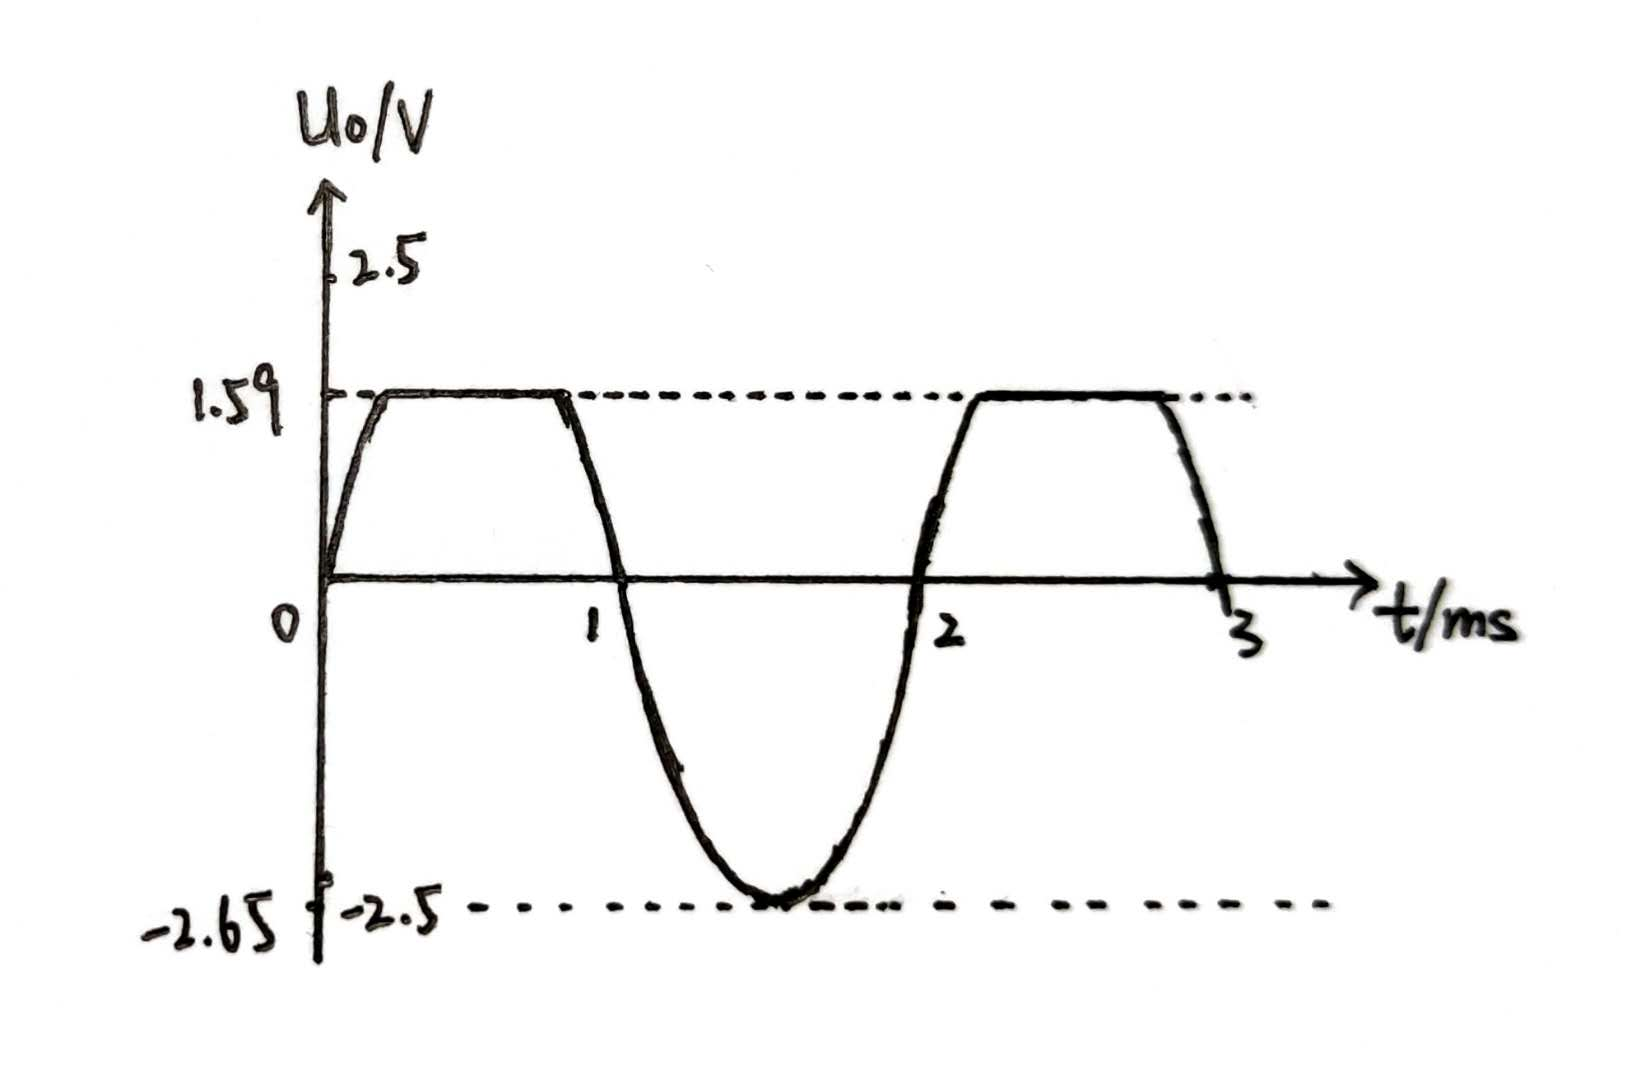
\includegraphics[width=7cm]{Exp3o}
 \caption{实验三输出波形}
 \label{fig:Exp3o}
\end{figure}
实验输出波形如图\ref{fig:Exp3o}所示。高值被削平,为$V_H=1.59\mr{V}$,低峰值为$V_L=-2.65\mr{V}$。
\par 被削平处的电压值应为电源电压加上二极管导通电压,即$1.00+0.5823=1.5823\mr{V}$,与实际值接近。
\par 将示波器输出模式改为$x - y$模式,测量$v_o - v_i$曲线。
\begin{figure}[H]
 \centering
 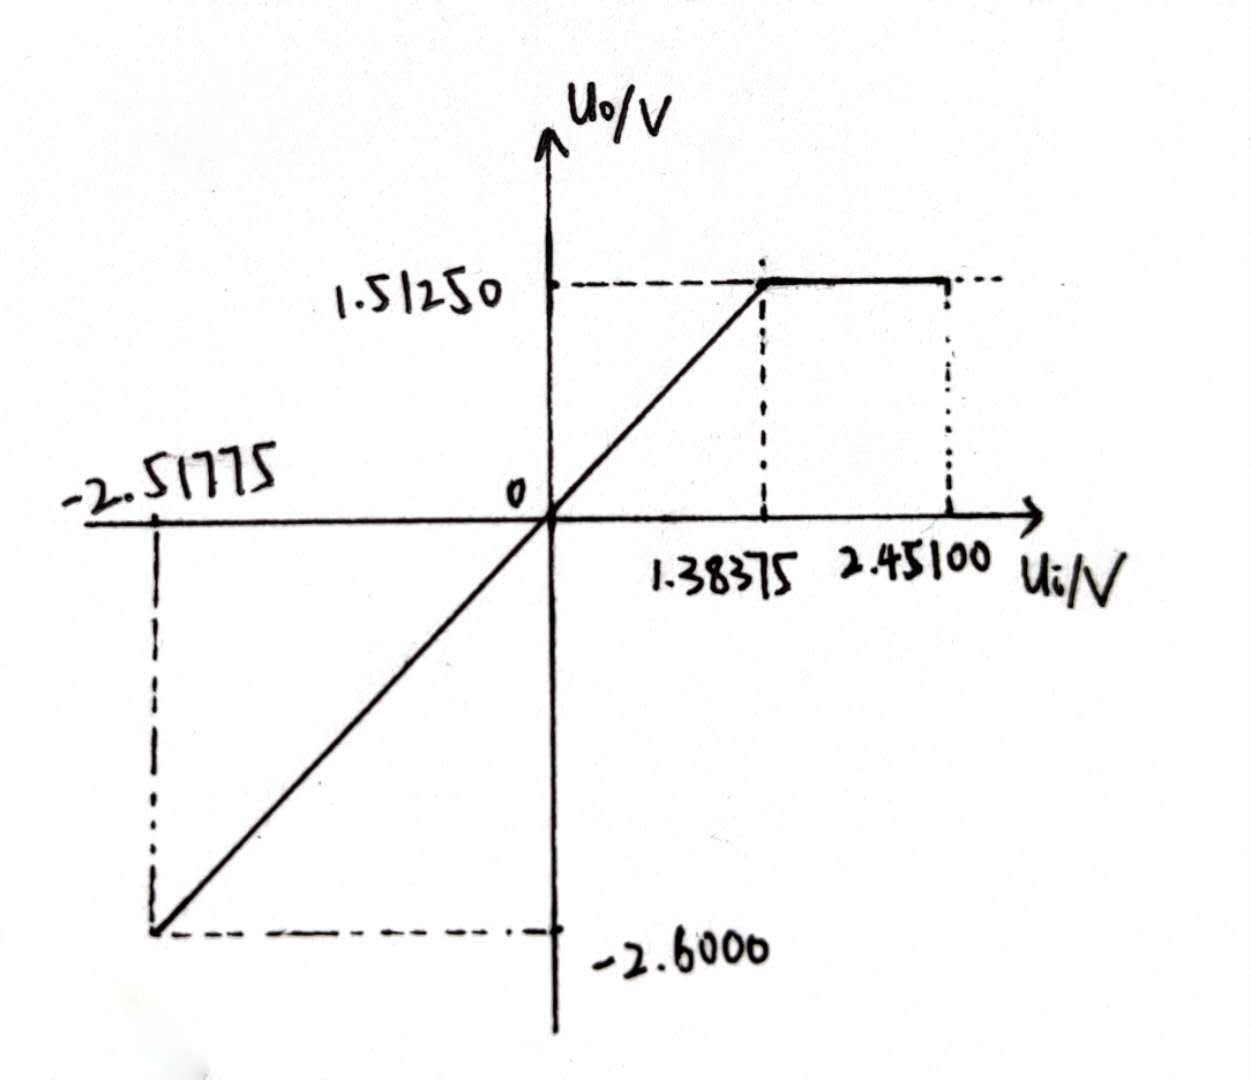
\includegraphics[width=6cm]{Exp3oxy}
 \caption{实验三输出波形,$x - y$模式}
 \label{fig:Exp3oxy}
\end{figure}
输出图像如图\ref{fig:Exp3oxy}所示。可见在$u_i$小于阈值电压$1.38375\mr{V}$时,$u_o$与$u_i$呈线性关系。若$u_i$大于阈值电压,那么$u_o$被限幅,$u_o$电压值不会继续上升,图线保持水平。
\subsection{实验四:稳压电路}
直流电压源$E=12\mr{V}$,接好电路连线再调整函数信号发生器的取值。在信号发生器显示有效值为$100\mr{mV_{rms}}$时,万用表实际测量的有效值为$94.81\mr{mV_{rms}}$。调整至万用表测量值为$100.06\mr{mV_{rms}}$时,函数信号发生器的标示有效值为$105.4\mr{mV_{rms}}$。
\par 改变万用表表笔所接位置,测得稳压管的静态反向电压为$V_Z=4.25\mr{V_{rms}}$,$R_1$两端电压为$V_1=99.41\mr{mV_{rms}}$,负载电阻$R_L$两端电压为$V_L=0.302\mr{mV_{rms}}$。
\par 由此计算:
\[ I_1=\frac{V_1}{R_1}=\frac{99.41\mr{mV}}{1\mr{k}\Omega}=99.41\mr{\upmu A},~
   I_L=\frac{V_L}{R_L}=\frac{0.302\mr{mV}}{2\mr{k}\Omega}=0.151\mr{\upmu A}.
   \]
\[
  I_Z=I_1-I_L=99.41\mr{\upmu A},~r=\frac{V_L}{I_Z}=3.04\Omega.
\]
下面求其等效电压源电压。假设输入负极接地,假设等效电源静态电压为$V_Z$,那么依照节点的KCL可以写出电路的方程:
\[ \frac{12-4.25}{1000}=\frac{4.25}{2000}+\frac{4.25-V_Z}{3.04} \]
由此解得:
\[ V_Z\approx4.233\mr{V}. \]
由此可以画出其等效电路:
\begin{figure}[H]
 \centering
 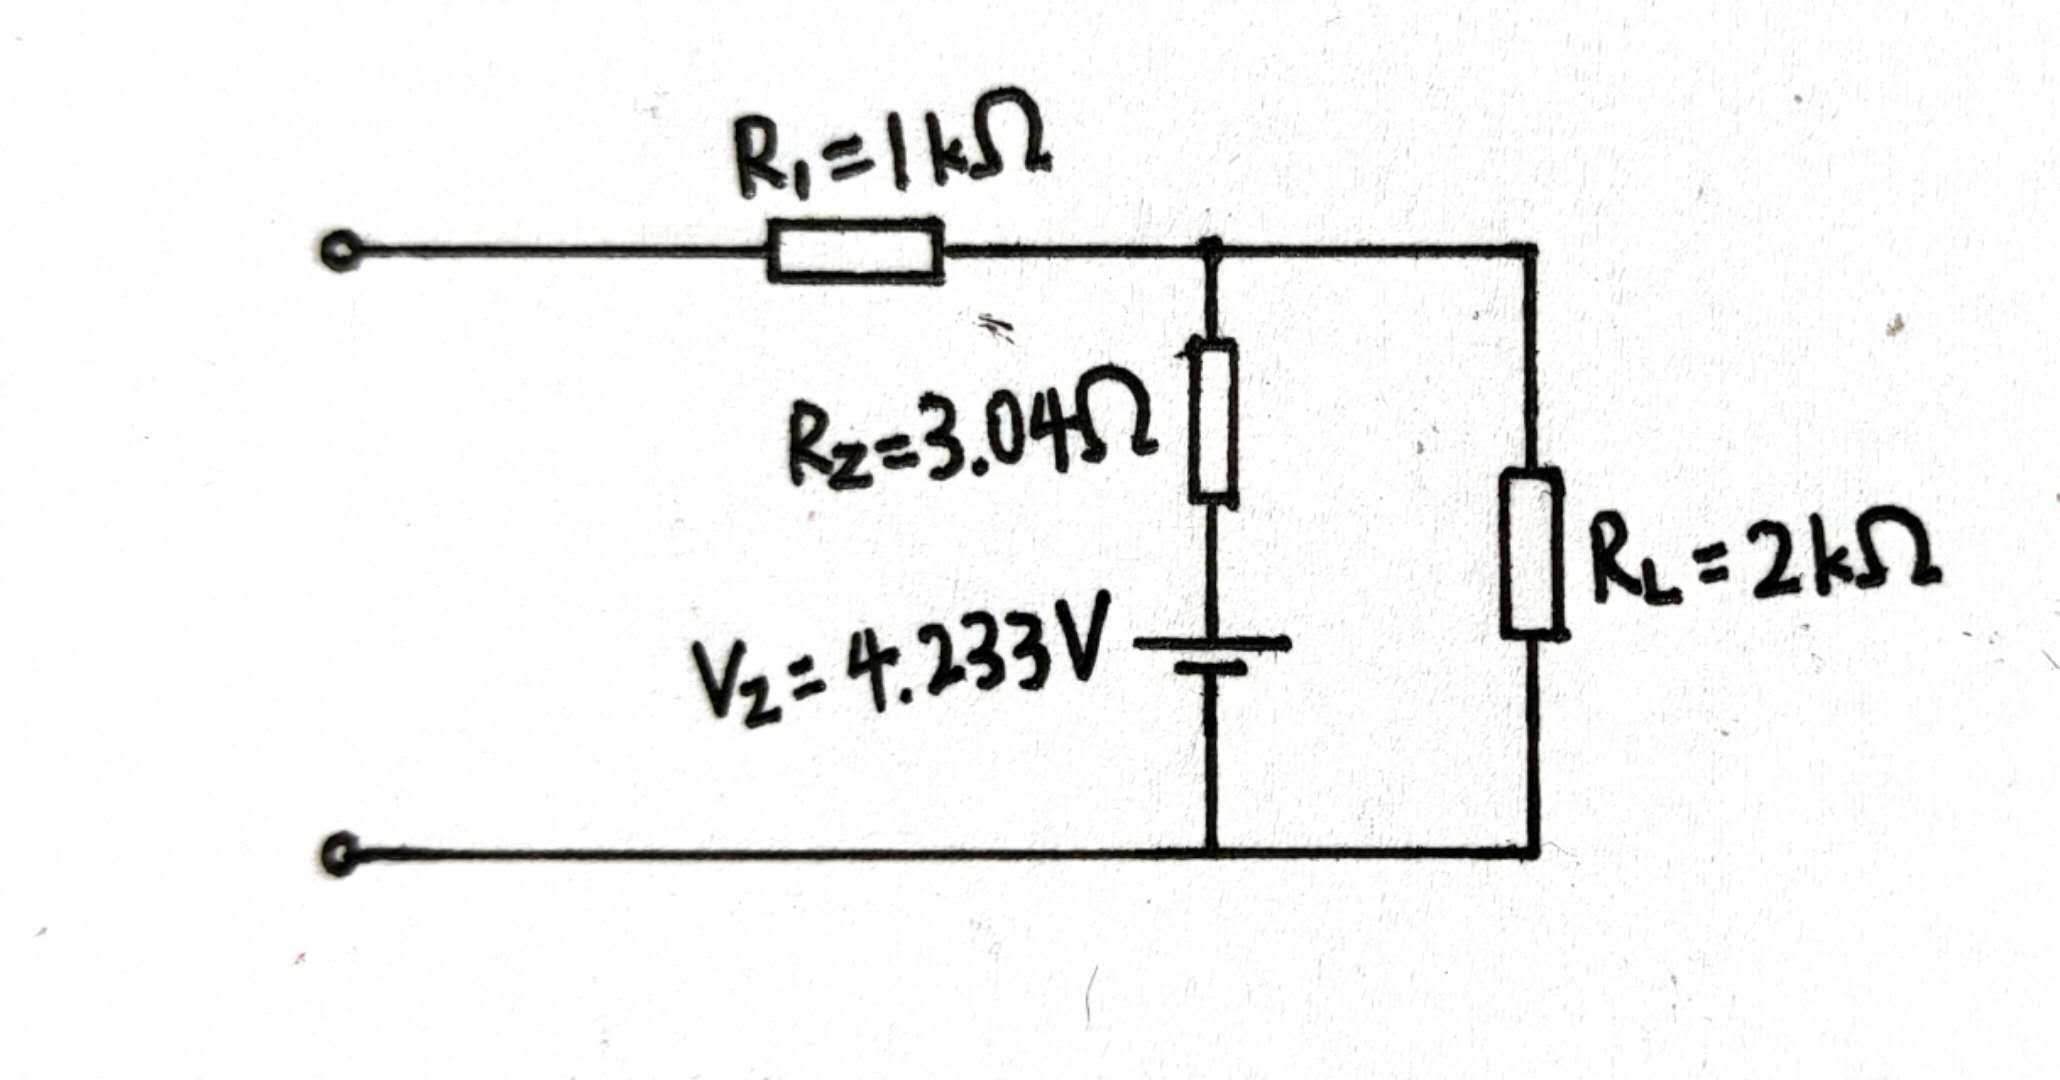
\includegraphics[width=8cm]{Exp4Circuit}
 \caption{实验四等效电路图}
 \label{fig:Exp4Circuit}
\end{figure}

\section{实验总结}
本次实验着重于二极管的性质和应用。经过若干个二极管实验,我们对二极管的整流、钳位、限幅(削波)有了更深入的认识。同时我们亲手验证了稳压二极管的稳压作用,并用交流小信号模型去求其等效电路。
\par 在任何规模的电路当中,二极管都是重要的组成成分,所以了解二极管的性质和常见用途,能有效地帮助我们理解复杂电路和自行设计电路。

\section{实验思考题}
\subsection{问题一}
二极管,对直流量,它相当于一个电压源,而对交流量,它等效成一个小电阻,这句话对吗?稳压管有何特性?

\textbf{答:}这句话需要添加更多的修饰条件,不完全正确。对于直流量,二极管导通时,可以采用恒压降模型,认为其管压降恒定,因此
可以近似成一个电压源,对于硅管,一般是$0.7V$,对于锗管,一般是$0.2V$。但电压很大时,应采用折线模型修正,看作一个有内阻的电压源。

对于交流分量,需要在小信号分析的前提下,采用小信号模型,其可以看作是一个小电阻,在只考虑交流量的情况下,有$r_d\approx\frac{V_T}{I_D}$,$V_T$为电压当量,$I_D$为Q点二极管电流。因此要求为小信号条件下,才可以看作为
小电阻。

稳压二极管,又称为齐纳二极管,这种管子杂质浓度很高,空间电荷区内的电荷密度很大,因而区域窄,容易形成强电场。当反向击穿时,反向电压波动不大即有较大的电流变化。但不能超过最大工作电流,否则进入反向特性转弯段,稳压特性消失,可能被烧毁。
\subsection{问题二}
说明稳压管并联稳压电路的稳压原理。

\textbf{答:}该电路的核心在于稳压管与并联。稳压管工作于反向击穿状态下时,其工作电压随电流变化很小,因此起到稳压作用。

而稳压管由于电压随电流变化很小,因此其动态电阻$r_z$非常小,因此将外界扰动导致的干路电流变化看作小信号。其在并联电路的作用下,由于稳压管动态电阻很小,小信号波动基本上会被
稳压管全部拾取,而稳压管电压随电流变化很小,因此稳压管在拾取了变化量后电压几乎维持不变,因此与之并联的输出电压也几乎不发生变化。

具体地说:当负载$R_L$一定时,如果$V_i$增大,则$V_z$增大,由于稳压二极管动态电阻很小,干路的电流基本上被其捕获,因此$R_1$上的压降增大,最终$V_o$几乎不变。
当$R_L$减小时,则干路路电流增大,因此干路压降增大,则$V_z$分压减小,最终$V_o$基本不变。反之亦然。
\end{document}
